\chapter{Stato dell'Arte}
\label{chap:Stato dell'Arte}

Questo capitolo esamina come il mondo dello sport stia attraversando una forte evoluzione, segnata dall'integrazione di nuove tecnologie. Di seguito viene introdotto, in particolare, il concetto di \textit{Sport 4.0}, necessario per capire il contesto dell'elaborato.  
\section{Sport 4.0}
\label{sec:sport4.0}

Questo nuovo paradigma, denominato \textit{Sport 4.0} \cite{sport4.0}, si ispira al concetto di Industria 4.0, con l'obiettivo di rivoluzionare le attività sportive sotto tutti i punti di vista. In particolare, le pratiche tradizionali vengono integrate con tecnologie quali \textit{Internet of Things}, \textit{Artificial Intelligence}, \textit{Machine Learning}, \textit{Augmented Reality} e \textit{Virtual Reality}.

\noindent Lo scopo è migliorare le prestazioni degli atleti, ottimizzare le strategie di gioco e coinvolgere i tifosi in nuove esperienze.

\noindent Le principali aree di applicazione sono infatti:
\begin{itemize}
    \item \textbf{Analisi delle Performance}: analisi delle prestazioni degli atleti come singoli e come squadra, con lo scopo di ottimizzare e migliorare le loro performance in gara.
    \item \textbf{Coinvolgimento dei Fan}: che ha l'obiettivo di offrire esperienze immersive e coinvolgenti ai tifosi, tramite l'integrazione di realtà aumentata e virtuale.
    \item \textbf{Infrastrutture Smart}: introduce il concetto di \textit{Internet of Things}, utilizzato per la gestione Smart delle strutture sportive. Con lo scopo di renderle più sostenibili da un punto di vista energetico e di aumentare la sicurezza dei tifosi.
    \item \textbf{Salute e Benessere}: si interessa di monitorare, tramite l'utilizzo di dispositivi specifici che raccolgono dati biometrici, le metriche di salute degli atleti permettendo quindi di controllare gli sportivi in maniera più approfondita e personalizzata.
  \end{itemize}
  

\noindent In sintesi, \textit{Sport 4.0} rappresenta una grande evoluzione per il mondo sportivo. Integrando tecnologie innovative che ottimizzano ogni aspetto delle attività, dall'allenamento alla competizione, fino all'esperienza dei tifosi.

\section{Analisi delle Performance}

Questo è uno degli ambiti più rivoluzionati da \textit{Sport 4.0}, grazie all'integrazione di software e hardware che hanno permesso un approccio \textit{Data-Driven} nell'analisi degli atleti. L'implementazione e l'utilizzo di Software di analisi video, come alcuni competitor successivamente presentati, consentono di estrarre da registrazioni di allenamenti e competizioni informazioni e statistiche dettagliate.



L'utilizzo di hardware, invece, come sensori biometrici e dispositivi indossabili, consente di monitorare molti più parametri, dalla precisione dei movimenti alla resistenza fisica. Di conseguenza, si ottimizzano le performance atletiche e si minimizza il rischio di infortuni.

\pagebreak


\subsection{Esempi}
\vspace{\baselineskip}
\subsubsection{Dispositivi Indossabili}
\begin{wrapfigure}{r}{0.4\textwidth}
    \centering
    \vspace{-10px}
    \frame{
\includegraphics[scale=0.033]{wearable_technology.jpg}}
    \caption{Wearable technology}
    \label{fig:Wearable technology}
\end{wrapfigure}

Dal 2016 ad oggi, a dominare i primi tre posti delle classifiche di tendenze fitness, sono stati i Wearable. Così definiti, sono dei dispositivi indossabili come smartwatch e fitness tracker, che permettono di rilevare dati relativi alla salute e all'attività fisica. Pensati inizialmente per un pubblico di professionisti nello sport, nel tempo si sono estesi anche verso una clientela più generica con la passione del fitness. Questa larga diffusione sul mercato è stata resa possibile dalle interfacce estremamente \textit{User-friendly}, che hanno reso i Wearable un must-have per chiunque voglia monitorare la propria attività fisica e il proprio benessere.


% I dispositivi indossabili, come gli smartwatch e i sensori biometrici, sono ampiamente utilizzati per monitorare in tempo reale le prestazioni degli atleti. Un esempio significativo è rappresentato da Catapult Sports leader nel settore di sensori wearable, che successivmente verrà presentato. L'utilizzo di dispositivi di monitoraggio delle prestazioni fisiche permette di raccogliere dati su frequenza cardiaca, distanza percorsa e altri parametri chiave. Questi dati sono fondamentali per aiutare gli atleti a ottimizzare l'intensità degli allenamenti e a prevenire infortuni, grazie all'analisi dei carichi di lavoro e dei pattern di movimento.


\subsubsection{Sistemi di Analisi Biomeccanica}
Gli sport di squadra si distinguono per un elevato tasso di tecnica e tattica. La pallavolo,  nello specifico, è uno sport dove la tecnica rappresenta una caratteristica discriminante nelle capacità di un giocatore. Per esempio, la realizzazione del fondamentale della schiacciata, richiede il coordinamento totale dell'atleta, partendo dalla sequenza dei passi (rincorsa), al salto, fino ad arrivare al movimento di braccia e colpo sulla palla con perfetta coordinazione spazio/temporale ed equilibrio. La biomeccanica si occupa proprio di analizzare le forze e l'efficacia dei singoli movimenti. Tramite algoritmi che utilizzano telecamere e sensori, elaborando anche lo scanner 3D dell'atleta, si può analizzare a 360 gradi ogni singola azione. Lo scopo di queste analisi è quello di aiutare staff ed allenatori nella creazione di allenamenti mirati alla correzione dei difetti rilevati.

    % utilizzano sensori avanzati e telecamere ad alta velocità per creare modelli 3D dei movimenti degli atleti. Questi sistemi sono fondamentali per studiare la biomeccanica del movimento e prevenire infortuni. Un esempio concreto è l'uso dei sistemi di cattura del movimento basati su marker, come quelli offerti da \textit{Xsens}, che permettono di stimare le forze muscolari, i contatti articolari e prevedere le forze di reazione al suolo durante le attività sportive. Questi dati permettono ai fisioterapisti di personalizzare i programmi di recupero, monitorando il movimento delle articolazioni durante la riabilitazione da infortuni.

\subsubsection{Software di Analisi Video}
\begin{wrapfigure}{r}{0.4\textwidth}
    \centering
    \vspace{-10px}
    \frame{
\includegraphics[scale=0.033]{video_analysis.jpg}}
    \caption{Video analysis}
    \label{fig:Video analysis}
\end{wrapfigure}

Alcuni Club calcistici inglesi, come Leicester FC e Southampton FC, utilizzano largamente software di analisi video. Questi applicativi permettono di analizzare le prestazioni dei giocatori per raggiungere risultati precisi. Vengono utilizzati, ad esempio, in fase di scouting. L'analisi costante di giocatori dilettanti delle squadre giovanili, infatti, fornisce alle società una banca dati di informazioni che possono aiutare il processo della ricerca di nuovi talenti. Allo stesso modo, vengono analizzati anche i giocatori che le società danno in prestito. Anche qui lo scopo è di seguirli a 360 gradi per tutto il periodo contrattuale.



\vspace{\baselineskip}
\section{Competitors}
\label{sec:competitor}

Dopo aver approfondito il concetto di Sport 4.0 ed in particolare le tecnologie legate all'analisi delle performance, segue una prima analisi di mercato. Questo passaggio identifica lo stato dell'arte, e comprende al meglio le preferenze degli utenti. Grazie a queste informazioni, è possibile delineare con maggiore precisione le direzioni di sviluppo della Web App, assicurando che soddisfi le esigenze degli utenti e che si differenzi dalle soluzioni attualmente disponibili.

I competitor sono divisi in due categorie principali: chi si concentra esclusivamente sulla \textit{video analysis} e chi la combina con l'uso di hardware integrativi, denominati \textit{Hybrid Systems}.





\noindent Di seguito vengono illustrate le due tipologie, analizzando alcune soluzioni per ognuna. Da qui sono inoltre presentati due prodotti verticali allo sport della pallavolo. Questo aiuterà a definire meglio, in seguito, le caratteristiche del progetto. 
\pagebreak


\subsection{Video Analysis}
Le applicazioni e i software di analisi video rappresentano uno strumento essenziale per lo studio delle performance sportive. Questi strumenti permettono di fornire dashboard interattive a staff ed allenatori per svolgere analisi specifiche. Inoltre, i sistemi più avanzati sono integrati con algoritmi di \textit{Computer Vision}, che permettono di raccogliere informazioni automaticamente, semplificandone ulteriormente l'uso. 
% di partite e allenamenti, fornendo funzionalità di tracciamento, annotazione e analisi dettagliata delle prestazioni.
\noindent Di seguito vengono presentati tre competitor che si concentrano esclusivamente sulla video analysis.


\subsubsection{Dartfish}
\textit{Dartfish} \cite{DartFish} è una soluzione che permette l'automazione di alcuni processi di analisi utilizzando modelli di \textit{Computer Vision}. Tramite algoritmi di \textit{pose estimation} e in alcuni casi di \textit{object tracking}, il software estrae informazioni dai video forniti. I dati raccolti vengono poi elaborati per fornire statistiche e grafiche utili all'utente finale. \textit{Dartfish} propone 3 soluzioni così suddivise: \textit{game analysis}, \textit{motion analysis} e \textit{HealthCare}. Questi prodotti, anche se con funzionalità differenti tra loro, hanno lo scopo comune di aiutare il lavoro degli analisti sportivi. \textit{Dartfish} non è indicato per l'utilizzo nell'ambito della pallavolo, non fornisce infatti modelli specifici per questo sport.
% permettono di rilevare pattern di gioco e attribuendo rating alle performance degli atleti. Grazie all'impiego di algoritmi di Computer Vision, \textit{Dartfish} processa grandi quantità di dati video, estrapolando \textit{insight} dettagliati relativi alle metriche di gioco. Funzionalità chiave del software includono il tracciamento di oggetti, l'analisi delle pose e la valutazione dettagliata delle performance, il tutto finalizzato all'ottimizzazione delle strategie e al miglioramento delle prestazioni sportive.

\subsubsection{LongoMatch}
\textit{LongoMatch} \cite{LongoMatch} - nato come progetto open source poi diventato proprietario - si concentra sull'analisi di eventi nei video. Infatti è utilizzato principalmente per la sua funzionalità di \textit{tagging}. Questa feature consente agli utenti di annotare azioni e momenti d'interesse durante la fase di analisi. L'interfaccia dell'app è personalizzabile dal singolo utente, permettendo agli analisti sportivi di creare \textit{dashboard} secondo le loro necessità. Un'altra delle caratteristiche specifiche di \textit{LongoMatch} è definita come "Drawing" (illustrata in figura \ref{fig:drawing_longo}) che permette di disegnare direttamente sui frame video, utile quando si vogliono sviluppare schemi di gioco. \textit{LongoMatch} risulta così essere un software versatile, ma allo stesso tempo complesso per utenti non esperti. Infatti, \textit{LongoMatch}, si ritrova ad essere una soluzione non sufficientemente \textit{user-friendly} per un utente amatoriale, ma allo stesso tempo con funzionalità troppo limitate per un team professionale.

\begin{figure}[htb]
    \centering 
\begin{subfigure}{0.33\textwidth}
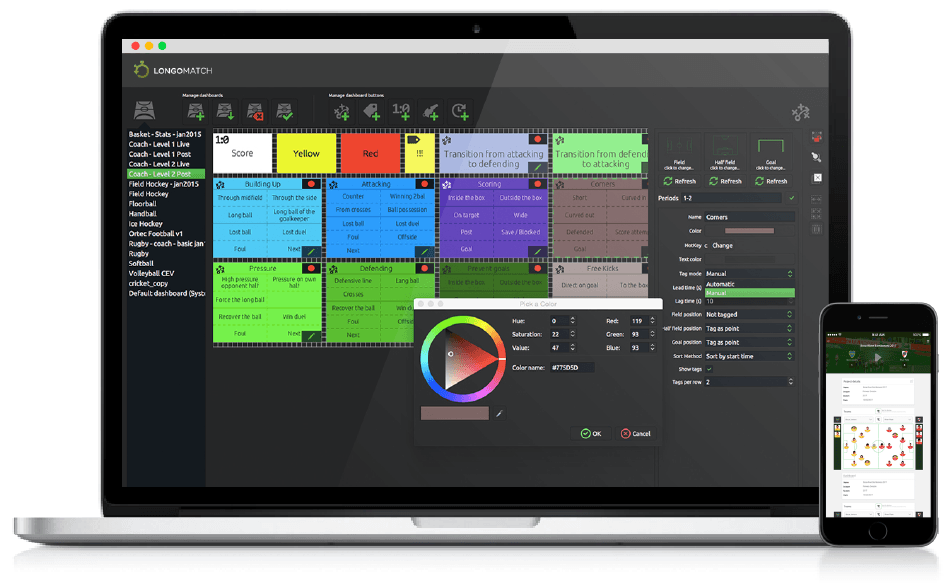
\includegraphics[width=\linewidth]{customize_longo.png}
\caption{Customization}
\label{fig:customization_longo}
\end{subfigure}\hfil
\begin{subfigure}{0.33\textwidth}
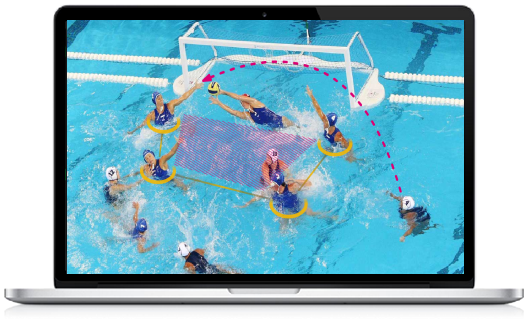
\includegraphics[width=\linewidth]{drawing_longo.png}
\caption{Drawing}
\label{fig:drawing_longo}
\end{subfigure}\hfil 
\begin{subfigure}{0.33\textwidth}
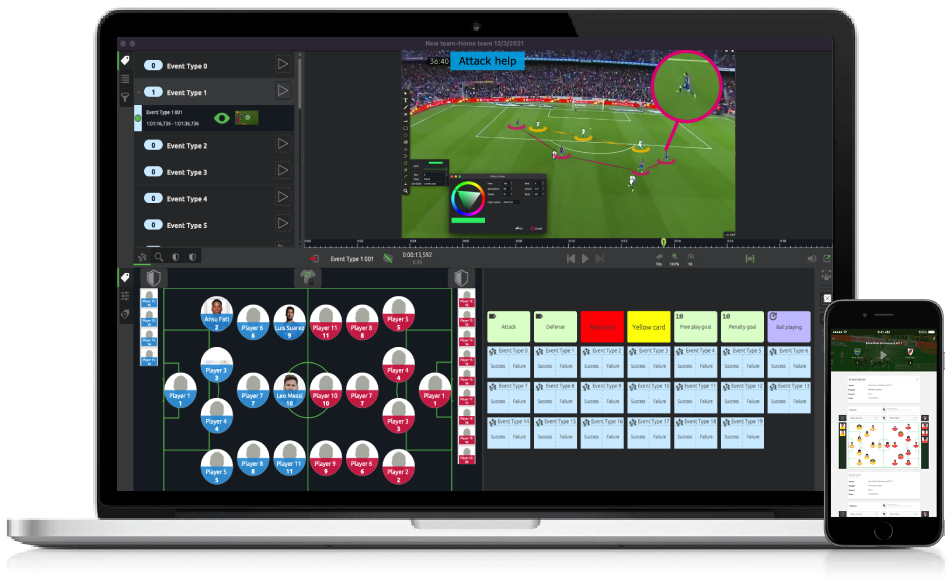
\includegraphics[width=\linewidth]{tagging_longo.png}
\caption{Tagging}
\label{fig:tagging_longo}
\end{subfigure}\hfil 
\caption{
\label{fig:analysis_competitor}LongoMatch Functionalities}
\end{figure}

\subsubsection{NAC Sport}
\textit{NAC Sport} \cite{NacSport} è un app con caratteristiche molto simili a quelle di \textit{LongoMatch}. Ciò che la distingue, è la possibiltà di effettuare analisi in \textit{realtime}, fornendo all'utente feedback istantanei. Inoltre supporta il riconoscimento tridimensionale di palla e giocatori, per avere un panorama a 360 gradi di un determinato evento. Come \textit{LongoMatch}, implementa funzionalità di tagging eventi tramite dashboard o shortcut da tastiera preimpostati. Implementa inoltre grafiche interattive, come ad esempio \textit{heatmaps}, per fornire ulteriori dettagli all'utente. Economicamente, \textit{NAC Sport} risulta essere più costoso rispetto ad altre alternative, proprio perchè è stato progettato per soddisfare le esigenze di un target professionale. Questi aspetti rendono \textit{NAC Sport} uno software completo, ma non adatto ad un bacino di utenti amatoriali.

\pagebreak

\subsection{Hybrid Systems}
Gli \textit{Hybrid Systems}, come dice la sigla stessa, combinano software di analisi video e tecnologie esterne. Alcuni esempi di hardware integrativi sono i dispositivi wearable, i sensori e le telecamere specializzate. Questi sistemi risultano estremamente efficienti perchè suddivisi in due fasi. Inizialmente, l'utilizzo di sensori permette di monitorare molti parametri che, successivamente, vengono utilizzati ed integrati nella fase di analisi video per avere risultati più precisi. 
\noindent Di seguito sono presentate ed illustrate 2 soluzioni leader nel settore.

\subsubsection{Hudl}
\label{subsubsec:hudl}
\begin{wrapfigure}{r}{0.48\textwidth}
    \centering
    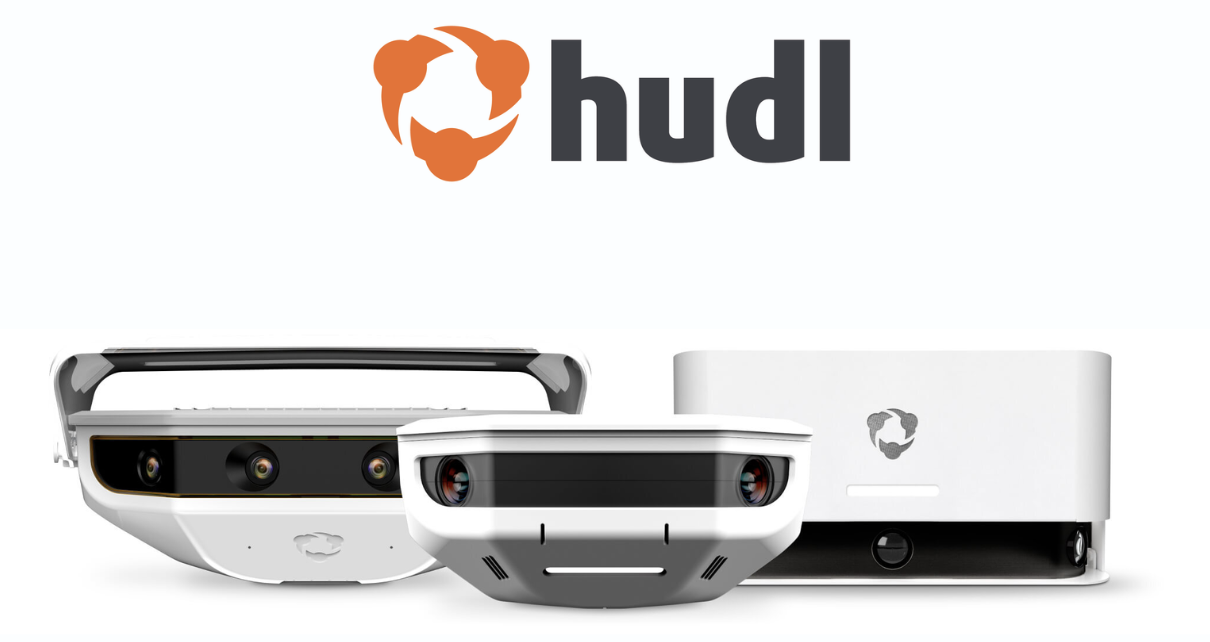
\includegraphics[scale=0.4]{hudl_focus.png}
    \caption{Hudl Focus}
    \label{fig:Hudl Focus}
\end{wrapfigure}
Hudl \cite{Hudl} è una piattaforma di analisi video sportiva, utilizzata da oltre \textit{8 milioni} di utenti registrati e \textit{230.000 squadre} in più di \textit{40 sport}, con \textit{16 milioni} di download dell'app.

\noindent Hudl offre una vasta gamma di prodotti innovativi per rispondere alle esigenze del mondo dello \textit{Sport 4.0}. I principali sono: \textit{Sportscode}, \textit{Volleymetrics}, \textit{Assist}, \textit{WIMU} e \textit{Hudl Focus}.

\noindent Proprio quest'ultimo è il servizio di punta dell'azienda, che integra l'analisi video con l'utilizzo di telecamere progettate da Hudl stessa.  In particolare l'azienda ha sviluppato software dedicati che permettono alle camere di seguire le azioni live in maniera automatica, offrendo una soluzione completamente \textit{hands-free}. Hudl Focus utilizza queste camere intelligenti per registrare ogni momento del gioco senza interventi manuali. Questo servizio è particolarmente utilizzato negli sport in cui il campo di gioco è ampio, ad esempio calcio o football americano.




\subsubsection{Catapult}
\label{subsubsec:catapult}
\begin{wrapfigure}{r}{0.48\textwidth}
    \centering
    \vspace{-15px}
    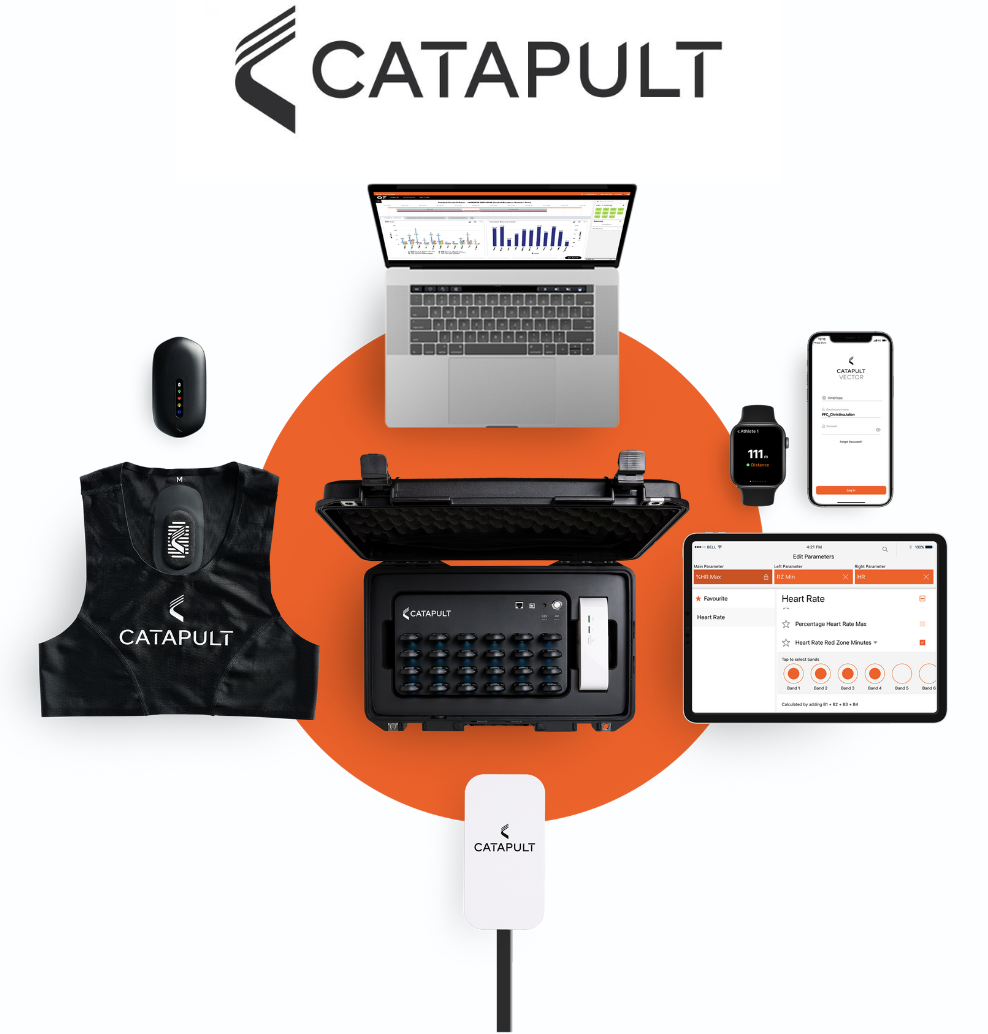
\includegraphics[scale=0.48]{catapult.png}
    \caption{Catapult Vector Core}
    \label{fig:Catapult Vector Core}
\end{wrapfigure}
Catapult \cite{Catapult} è una piattaforma leader nel monitoraggio e nell'analisi sportiva, utilizzati da oltre \textit{4.200 squadre} in più di \textit{40 sport} in tutto il mondo. Uno dei loro prodotti di punta è \textit{Vector Core}.

Questa soluzione fornisce pettorine con tecnologie GPS/GNSS  per tracciare i movimenti degli atleti, fornendo dati in \textit{realtime} ma anche post-sessione. Il prodotto ha riscosso grande successo perchè facile da configurare e offre un'ampia gamma di metriche per l'analisi delle prestazioni fisiche. 

\noindent Le caratteristiche principali di Vector Core includono:
\begin{itemize}
    \item \textit{Tracciamento integrato indoor e outdoor}
    \item \textit{Tecnologia GPS/GNSS a 10 Hz}
    \item \textit{Analisi inerziale del movimento}
    \item \textit{Compatibilità con monitoraggio della frequenza cardiaca}
    \item \textit{Reportistica dettagliata con oltre 200 parametri live e 1.800 parametri post-sessione}
\end{itemize}

\subsection{Volleyball Specific}
Alcune aziende si sono specializzate nel fornire soluzioni verticali per specifici sport, come la pallavolo. Di seguito analizziamo due esempi rilevanti.

\subsubsection{DataVolley 4.0}
DataVolley 4.0 \cite{Data-Volley4.0} è uno dei prodotti di riferimento nella pallavolo internazionale ed è sviluppato dall'azienda Data Project. Il software è progettato per la raccolta e analisi di dati di partite ed allenamenti. Il suo punto di forza risiede nell'interfaccia per la raccolta dei dati (molto simile alla stenografia) e nelle successive funzioni che permettono di generare report e statistiche relative alle squadre e ad ogni singolo giocatore associando anche il video. L'applicazione è focalizzata in particolare alla raccolta dei dati delle performance e non all'analisi dei singoli fondamentali (e quindi la tattica). Inoltre richiede un po' di addestramento per imparare ad utilizzarlo, per cui utenti amatoriali finiscono per non farne uso anche se esistono versioni economiche.


\subsubsection{BallTime}
BallTime \cite{BallTime} è una startup NewYorkese che sfrutta modelli di Computer Vision per l'analisi video. In particolare i modelli di ML riescono a:
\begin{itemize}
    \item Riconoscere e distinguere i singoli giocatori
    \item Tracciare la palla
    \item Analizzare pattern di gioco
    \item Riconoscere azioni e segnare il risultato
\end{itemize} 

La startup, nata a Settembre 2022, fornisce una web app completa, ma ancora in costante sviluppo. Infatti questa soluzione sta introducendo le funzionalità di volta in volta guidata dalla domanda. L'approccio innovativo e soprattutto \textit{user-friendly}, il prezzo contenuto e l'attività di marketing che l'azienda sta sviluppando, rendono \textit{BallTime} una soluzione competitiva dove le alternative dovranno puntare su funzioni diverse o strategie di creazione di comunità.

